\documentclass[11pt,a4paper]{article}

\usepackage[T1]{fontenc}
\usepackage[utf8]{inputenc}
\usepackage{mathptmx}
\usepackage{courier}
\usepackage[margin=2.5cm]{geometry}
\usepackage{amsmath}
\usepackage{booktabs}
\usepackage{graphicx}
\usepackage{xcolor}
\usepackage[numbers,sort&compress]{natbib}
\usepackage{xurl}
\usepackage[hidelinks]{hyperref}
\hypersetup{pdftitle={Told the Price, Buying Everything: Small LLM Agents in Cost-Aware Evidence Acquisition for Kepler Candidate Vetting},pdfauthor={Muzammal Hussain}}
\usepackage{caption}
\captionsetup{font=small,labelfont=bf}

\newcommand{\code}[1]{\texttt{#1}}
\setlength{\emergencystretch}{3em}

\title{\textbf{Told the Price, Buying Everything:\\Small LLM Agents in Cost-Aware Evidence Acquisition\\for Kepler Candidate Vetting}}
\author{Muzammal Hussain\\
\small Independent researcher, Glasgow, United Kingdom\\
\small \href{mailto:muzammal@masmatixinnovations.co.uk}{muzammal@masmatixinnovations.co.uk}\\
\small ORCID: \href{https://orcid.org/0009-0001-2570-5686}{0009-0001-2570-5686}}
\date{\small November 2026}

\begin{document}
\maketitle

\begin{abstract}
\noindent
An agent that vets a transit signal can look at more evidence, but each look has a cost. We built a benchmark in
which a policy starts from four cheap signal metrics of a Kepler object of interest (KOI) and may buy three further
evidence groups (transit geometry, fit quality, stellar context) before a fixed classifier predicts the DR25
Supplemental disposition. On 5,323 KOIs with host-star-grouped cross-validation, buying everything gives ROC AUC
0.867 and balanced accuracy 0.799. A rule that stops once the classifier is 85\% confident spends 29\% less
(mean cost 3.83 of 5.4) for the same balanced accuracy (difference $-0.001$, 95\% CI $[-0.002, 0.000]$) and an
AUC 0.003 lower; a cost-weighted information-gain order did no better than a fixed order. Two small local LLM agents
(\code{qwen2.5:3b}, \code{llama3.1:8b}) given the same choice, the classifier's current probability and the costs,
never stopped early: on 300 KOIs they bought every group in all 300 episodes, also when the prompt said that stopping
is free and that evidence should be bought only if it could change the label, and on 47 KOIs whose label was already
clear after the first group. Under a tighter budget \code{qwen2.5:3b} asked for an unaffordable group in every
episode. Budget discipline in such agents should be enforced by the environment, not delegated to the model.
\end{abstract}

\section{Introduction}

Vetting a transit signal means deciding whether it is a planet candidate or a false positive, and the evidence for
that decision comes in groups of different cost: the signal itself, a transit model fit, diagnostics of that fit and
the properties of the host star. Active feature acquisition studies how to buy such evidence sequentially, trading
the cost of each feature against the accuracy of the final prediction~\cite{saar2009afa,aronsson2026afa}. Tool-using
LLM agents are now asked to make the same kind of choice in many domains: what to look up next, and when to stop.

We ask three questions on a fixed, public task. (1) How close can sequential acquisition get to full-information
performance at lower cost? (2) Does an information-gain order beat a fixed or random order at the same budget?
(3) Does a small local LLM, given the costs and the classifier's current confidence, choose evidence economically?
The task is deliberately simple, so that the LLM's only job is the acquisition decision: the label always comes from
the same classifier, whichever policy chose the evidence.

The target is the disposition in the Kepler DR25 Supplemental table~\cite{thompson2018dr25,nea2018koidr25}. It
combines automated and human vetting; predicting it is a benchmark of agreement with that catalogue, not a
confirmation of planets.

\section{Related work}

\paragraph{Kepler candidate vetting.} The DR24 and DR25 catalogues were produced by the Robovetter, an expert system
of hand-tuned tests on the light curve and pipeline diagnostics~\cite{coughlin2016dr24,thompson2018dr25}. The
Autovetter classified the same threshold-crossing events with a random forest on pipeline attributes
\cite{mccauliff2015autovetter}, and Astronet trained a convolutional network on the folded light curves
\cite{shallue2018astronet}. All three see every feature for every signal; we ask instead which features are worth
paying for, and use a deliberately simple classifier so that the acquisition decision is the only variable.

\paragraph{Cost-aware acquisition and tool use.} Active feature acquisition buys features per instance to trade
cost against accuracy~\cite{saar2009afa,aronsson2026afa}. For LLM agents the analogous failure is tool overuse:
calling tools when the answer is already available, which SMART~\cite{qian2025smart} reduces by training agents to
recognise when a tool is needed. Our agents do not choose between a tool and their own knowledge but between more
evidence and stopping, and we test whether a prompt alone, with the costs and the classifier's confidence in view, is
enough.

\section{Method}

\paragraph{Data.} We query the NASA Exoplanet Archive table \code{q1\_q17\_dr25\_sup\_koi} and join the DR25 transit
fits; KOIs labelled \code{CANDIDATE} (1) or \code{FALSE POSITIVE} (0) with usable features are kept: 5,323 KOIs
(1,377 candidates) around 5,158 host stars. The prior pipeline disposition, disposition scores, false-positive flags
and comments are excluded from the inputs.

\paragraph{Evidence groups and costs.} Signal metrics (model SNR, number of transits, maximum multiple- and
single-event statistics; cost 1.0), transit geometry (period, duration, depth, impact parameter, radius ratio, stellar
density from the fit; 1.2), fit quality (odd--even depth significance; 1.4) and stellar context (effective
temperature, $\log g$, metallicity, radius, mass; 1.8). Every episode starts with the signal metrics; buying all four
groups costs 5.4. Costs are normalised units, not telescope time.

\paragraph{Classifier.} For each of the 15 subsets of groups that contain the signal metrics we fit a
class-balanced logistic regression with median imputation (plus missingness indicators) and standardisation. Five
outer folds are built with stratified group k-fold on the host star (\code{kepid}), so no star appears in both
training and test data. A policy decides which groups to buy; the classifier for the bought subset gives the
probability and the label.

\paragraph{Policies.} \emph{Signal only} buys nothing more. \emph{Full information} buys everything. \emph{Fixed}
buys geometry, fit quality and stellar context in that order; \emph{random} in a random order. Both stop once the
classifier's confidence $\max(p, 1-p)$ reaches 0.85 or the budget is spent. \emph{Adaptive} uses the same stopping
rule but picks the group with the largest expected entropy reduction per unit cost, estimated on a held-out
calibration split of the training folds for each confidence bucket. Rule policies run at budgets 5.4 (everything
affordable) and 4.0.

\paragraph{LLM agents.} \code{qwen2.5:3b}~\cite{qwen2025qwen25} and \code{llama3.1:8b}~\cite{grattafiori2024llama3}
run through Ollama with temperature 0 and JSON output on a laptop. At each step the agent sees the available groups,
their costs and field names, the groups already bought, the remaining budget, the classifier's current probability
and the visible feature values, and returns \code{request} with a group or \code{stop}. The environment refuses a
request the budget cannot pay for. A \emph{neutral} prompt states these rules; a \emph{cost-aware} prompt adds that
the objective is the right label at the lowest cost, that stopping is not penalised, that the probability comes from
a calibrated classifier, and that a group should be bought only if it could change the label. Because each episode
takes several model calls, the agents run on the first 300 test KOIs of fold 1 (86 candidates); the rule policies are
reported on all 5,323 KOIs and, for comparison, on the same 300.

\paragraph{Metrics.} ROC AUC, balanced accuracy and mean acquisition cost. Intervals are 95\% percentile intervals
from 1,000 bootstrap resamples of host stars~\cite{efron1993bootstrap}; differences are paired on the same KOIs.

\section{Results}

\begin{table}[t]
\centering
\small
\caption{Rule policies on all 5,323 KOIs (out-of-fold predictions). Cost: mean normalised acquisition cost (maximum
5.4). Differences to full information are paired; 95\% host-star bootstrap intervals in brackets.}
\label{tab:main}
\setlength{\tabcolsep}{4pt}
\begin{tabular}{llcccc}
\toprule
Budget & Policy & Cost & ROC AUC & $\Delta$AUC vs full & Balanced acc. \\
\midrule
-- & Signal only & 1.00 & 0.805 [0.794, 0.817] & $-0.061$ [$-0.072$, $-0.052$] & 0.744 \\
-- & Full information & 5.40 & 0.867 [0.857, 0.877] & -- & 0.799 \\
\midrule
5.4 & Fixed & 3.86 & 0.863 [0.853, 0.874] & $-0.003$ [$-0.006$, $-0.002$] & 0.799 \\
 & Random & 4.03 & 0.864 [0.853, 0.874] & $-0.003$ [$-0.005$, $-0.001$] & 0.798 \\
 & Adaptive & 3.83 & 0.863 [0.853, 0.874] & $-0.003$ [$-0.005$, $-0.002$] & 0.799 \\
\midrule
4.0 & Fixed & 2.77 & 0.858 [0.847, 0.868] & $-0.009$ [$-0.014$, $-0.005$] & 0.794 \\
 & Random & 3.02 & 0.861 [0.850, 0.871] & $-0.006$ [$-0.010$, $-0.002$] & 0.797 \\
 & Adaptive & 2.97 & 0.861 [0.852, 0.871] & $-0.005$ [$-0.008$, $-0.003$] & 0.795 \\
\bottomrule
\end{tabular}
\end{table}

\paragraph{Sequential acquisition saves about 30\% at almost no loss.} The signal metrics alone give AUC 0.805; all
four groups give 0.867 (Table~\ref{tab:main}). Stopping at 85\% confidence, the adaptive policy spent 3.83 on
average, 29\% less than full information, with the same balanced accuracy (difference $-0.001$ [$-0.002$, $0.000$])
and an AUC 0.003 lower. It stopped after the signal metrics for 1,332 KOIs (25\%) and bought everything for 3,045
(57\%). At budget 4.0 it spent 2.97 and lost 0.005 AUC.

\paragraph{The information-gain order equals the fixed order.} Adaptive and fixed policies differ by less than 0.001
AUC at budget 5.4 (paired interval $[-0.001, 0.001]$). When the adaptive policy bought a second group, it chose
transit geometry for 3,968 of 3,991 KOIs, which is also the fixed order's first choice; the saving comes from the
stopping rule, not from the order.

\begin{figure}[t]
  \centering
  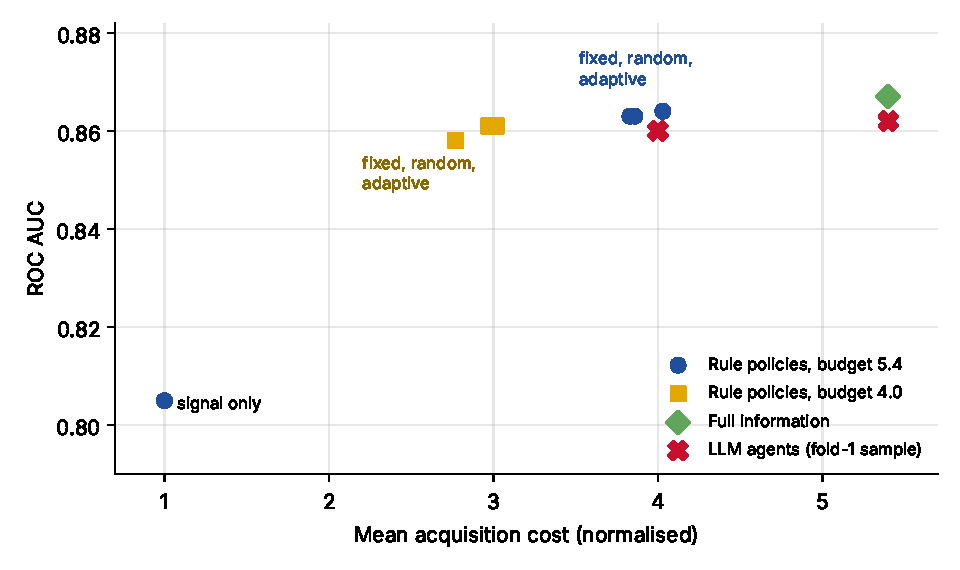
\includegraphics[width=0.78\linewidth]{figures/fig_cost_auc.pdf}
  \caption{ROC AUC against mean acquisition cost. Rule policies and full information: all 5,323 KOIs. LLM agents
  (both models, both prompts at budget 5.4; cost-aware prompt at budget 4.0): the 300 fold-1 KOIs, on which full
  information scores 0.862.}
  \label{fig:cost}
\end{figure}

\paragraph{The LLM agents buy everything they can.} With the neutral prompt and budget 5.4, both models requested
all three remaining groups in all 300 episodes and never chose \code{stop}, so their cost was 5.40 and their
predictions were identical to full information (Figure~\ref{fig:cost}). The cost-aware prompt changed nothing:
\code{llama3.1:8b} again bought everything in 300 of 300 episodes and \code{qwen2.5:3b} in 300 of 300. On the same
300 KOIs the adaptive rule spent 4.33 for a balanced accuracy of 0.801 against the agents' 0.798. On 47 of the 300
KOIs the classifier was already at least 85\% confident after the signal metrics; the agents bought three more groups
for every one of them. The models also ignored the prices when choosing the order: \code{qwen2.5:3b} bought stellar
context, the most expensive group, second in every episode.

\paragraph{A tighter budget is spent, not respected.} At budget 4.0 with the cost-aware prompt, both models spent
exactly 4.0 in every episode (signal metrics, transit geometry and stellar context). \code{qwen2.5:3b} then asked for
a group it could not pay for in all 300 episodes, and the environment's budget guard ended the episode; it never
stopped by itself. Spending the whole budget did not buy accuracy: by taking stellar context instead of fit quality,
the agents reached a balanced accuracy of 0.785 on these KOIs, against 0.798 with full information and 0.795 for the
fixed rule, which spent 3.05.

\section{Discussion}

\paragraph{What the agents did not use.} The agents were given exactly the signal a good stopping rule needs, the
classifier's current probability, and an explicit instruction that stopping is free. They behaved as if more evidence
were always better. One reading is that small instruction-tuned models treat a list of available tools as a list of
things to do; another is that a probability of 0.9 does not register as ``enough''. Either way the behaviour is a
property of the agent, not of the task: a one-line threshold rule in the environment recovers almost all of the saving.

\paragraph{Where to put cost control.} In this benchmark the acquisition decision was the only thing the LLM
controlled, and leaving it to the model cost 25\% more than the threshold rule on the same 300 KOIs (5.40 against
4.33), without any gain in accuracy. Agents that call paid or slow tools should enforce
budgets and stopping rules in the environment, and report cost next to accuracy so that this behaviour is visible.

\paragraph{Why the order did not matter.} With only three optional groups and transit geometry the most informative
by a wide margin, any reasonable order begins with it, so the information-gain estimate had little to choose. Richer
evidence menus, where groups are closer in value and cost, are needed to test acquisition order itself.

\section{Limitations}

The target is a catalogue disposition, not physical truth. The classifier is a linear model on tabular features;
light curves and pixel data were not used, and a stronger model might change which groups are worth buying. Costs
are normalised and chosen by us, not measured. The LLM agents were run on 300 KOIs from one fold, once each at
temperature 0, with two prompts and two small models; larger models or a prompt that shows the expected value of each
group may behave differently. Because the classifier, not the agent, gives the label, the benchmark tests the
acquisition decision only.

\section{Conclusion}

On Kepler DR25 KOIs a simple confidence threshold cuts the evidence cost by 29\% at the same balanced accuracy, and an
information-gain order adds nothing over a fixed order. Two small local LLM agents, given the costs, the classifier's
confidence and an instruction to save, bought every group they could in every episode. Cost control for such agents
belongs in the environment.

\section*{Code and data availability}

Code, tests, per-KOI predictions and acquisition traces for every policy and agent run are at
\url{https://github.com/MHKhan50/exovet-agentbench}. The KOI table is not redistributed; the pipeline downloads it from
the NASA Exoplanet Archive TAP service and records the query, retrieval time, row count and SHA-256. Code is released
under the MIT licence and archived on Zenodo at \href{https://doi.org/10.5281/zenodo.24407523}{doi:10.5281/zenodo.24407523} (all versions).

\bibliographystyle{plainnat}
\bibliography{references}

\end{document}
